%!TEX program = xelatex
\documentclass[12pt, a4paper]{article}

\usepackage[dvipsnames]{xcolor}

\usepackage{fancyhdr}
\usepackage{extramarks}
\usepackage{amsmath}
\usepackage{amsthm}
\usepackage{amsfonts}
\usepackage{tikz}
\usepackage[plain]{algorithm}
\usepackage{algpseudocode}

\usepackage{ctex}
\usepackage{indentfirst}
\usepackage{wrapfig}
\usepackage{upgreek}
\usepackage{subfigure}
\ctexset {today=old}
\usetikzlibrary{automata,positioning,shapes.geometric,arrows.meta,patterns,calc}
\numberwithin{equation}{section}

%
% Basic Document Settings
%

\topmargin=-0.25in
\evensidemargin=0in
\oddsidemargin=0in
\textwidth=6.5in
\textheight=9.2in
\headsep=0.25in

\linespread{1.1}

\pagestyle{fancy}
\lhead{\hmwkAuthorName}
\chead{\hmwkClass : \hmwkTitle}
\rhead{\firstxmark}
\lfoot{\lastxmark}
\cfoot{\thepage}

\renewcommand\headrulewidth{0.4pt}
\renewcommand\footrulewidth{0.4pt}

\setlength{\parindent}{2em}  % 2em代表首行缩进两个字符

%
% Create Problem Sections
%

\newcommand{\enterProblemHeader}[1]{
    \nobreak\extramarks{}{Problem \arabic{#1} continued on next page\ldots}\nobreak{}
    \nobreak\extramarks{Problem \arabic{#1} (continued)}{Problem \arabic{#1} continued on next page\ldots}\nobreak{}
}

\newcommand{\exitProblemHeader}[1]{
    \nobreak\extramarks{Problem \arabic{#1} (continued)}{Problem \arabic{#1} continued on next page\ldots}\nobreak{}
    \stepcounter{#1}
    \nobreak\extramarks{Problem \arabic{#1}}{}\nobreak{}
}

% \setcounter{secnumdepth}{0}
\newcounter{partCounter}
\newcounter{homeworkProblemCounter}
\setcounter{homeworkProblemCounter}{0}
% \nobreak\extramarks{Problem \arabic{homeworkProblemCounter}}{}\nobreak{}

%
% Homework Problem Environment
%
% This environment takes an optional argument. When given, it will adjust the
% problem counter. This is useful for when the problems given for your
% assignment aren't sequential. See the last 3 problems of this template for an
% example.
%
\newenvironment{homeworkProblem}[1][-1]{
    \ifnum#1>0
        \setcounter{homeworkProblemCounter}{#1}
    \fi
    \section{Problem \arabic{homeworkProblemCounter}}
    \setcounter{partCounter}{1}
    \enterProblemHeader{homeworkProblemCounter}
}{
    \exitProblemHeader{homeworkProblemCounter}
}

%
% Homework Details
%   - Title
%   - Due date
%   - Class
%   - Section/Time
%   - Instructor
%   - Author
%

\newcommand{\hmwkTitle}{Rigid Body Mechanics}
\newcommand{\hmwkDueDate}{\today}
\newcommand{\hmwkClass}{University Physics}
\newcommand{\hmwkClassTime}{}
\newcommand{\myUniversiy}{Wuhan University}
\newcommand{\hmwkAuthorName}{\textbf{Lai Wei}}

%
% Title Page
%

\title{
    \vspace{2in}
    \textmd{\textbf{\hmwkClass:\ \hmwkTitle}}\\
    \normalsize\vspace{0.1in}\small{Date: \hmwkDueDate}\\
    \vspace{0.1in}\large{\textit{\myUniversiy}}
    \vspace{3in}
}

\author{\hmwkAuthorName}
\date{}

\renewcommand{\part}[1]{\textbf{\large Part \Alph{partCounter}}\stepcounter{partCounter}\\}

%
% Various Helper Commands
%

% Useful for algorithms
\newcommand{\alg}[1]{\textsc{\bfseries \footnotesize #1}}

% % For derivatives
% \newcommand{\deriv}[1]{\frac{\mathrm{d}}{\mathrm{d}x} (#1)}

% For partial derivatives
\newcommand{\pderiv}[2]{\frac{\partial}{\partial #1} (#2)}

% Integral dx
\newcommand{\dx}{\mathrm{d}x}

% Alias for the Solution section header
\newcommand{\solution}{\textbf{\large Solution}}

% Probability commands: Expectation, Variance, Covariance, Bias
\newcommand{\E}{\mathrm{E}}
\newcommand{\Var}{\mathrm{Var}}
\newcommand{\Cov}{\mathrm{Cov}}
\newcommand{\Bias}{\mathrm{Bias}}

% 我的newcommand
\newcommand{\degree}{^{\circ}}
\newcommand{\arrow}{-{Stealth[length=4mm,width=2mm]}}
\newcommand{\rmd}{\mathrm{~d}}
\newcommand{\deriv}[2]{\frac{\rmd #1}{\rmd #2}}
\renewcommand{\parallel}{\mathrel{/\mskip-2.5mu/}}

\begin{document}

\maketitle

\pagebreak

% 设置页码格式是罗马数字
\pagenumbering{roman}

% 生成目录
\tableofcontents

\pagebreak

% 设置页码格式是阿拉伯数字
\pagenumbering{arabic}

\pagebreak

\section{刚体的定轴转动}

\subsection{刚体}

\subsubsection{定义}

    在外力作用下,形状和大小都不发生变化的物体。(任意两质点间距离保持不变的特殊质点组。)

    \begin{enumerate}
        \item 刚体是理想模型;
        \item 刚体模型是为简化研究问题而引进的。
    \end{enumerate}

\subsubsection{平动}

    刚体中所有点的运动轨迹都保持完全相同。(各点的状态一样)

    刚体上任意一点的运动可以代表整个刚体的运动。(刚体平动的运动规律和与质点的运动规律相同)

\subsection{转动}

    分为\textbf{定轴转动}和\textbf{非定轴转动}。

    刚体的一般运动可以看作“随质心的平动”和“绕质心的转动”的合成。

\subsubsection{刚体转动的角速度和角加速度}

    \begin{wrapfigure}{r}{4cm}
        \centering
        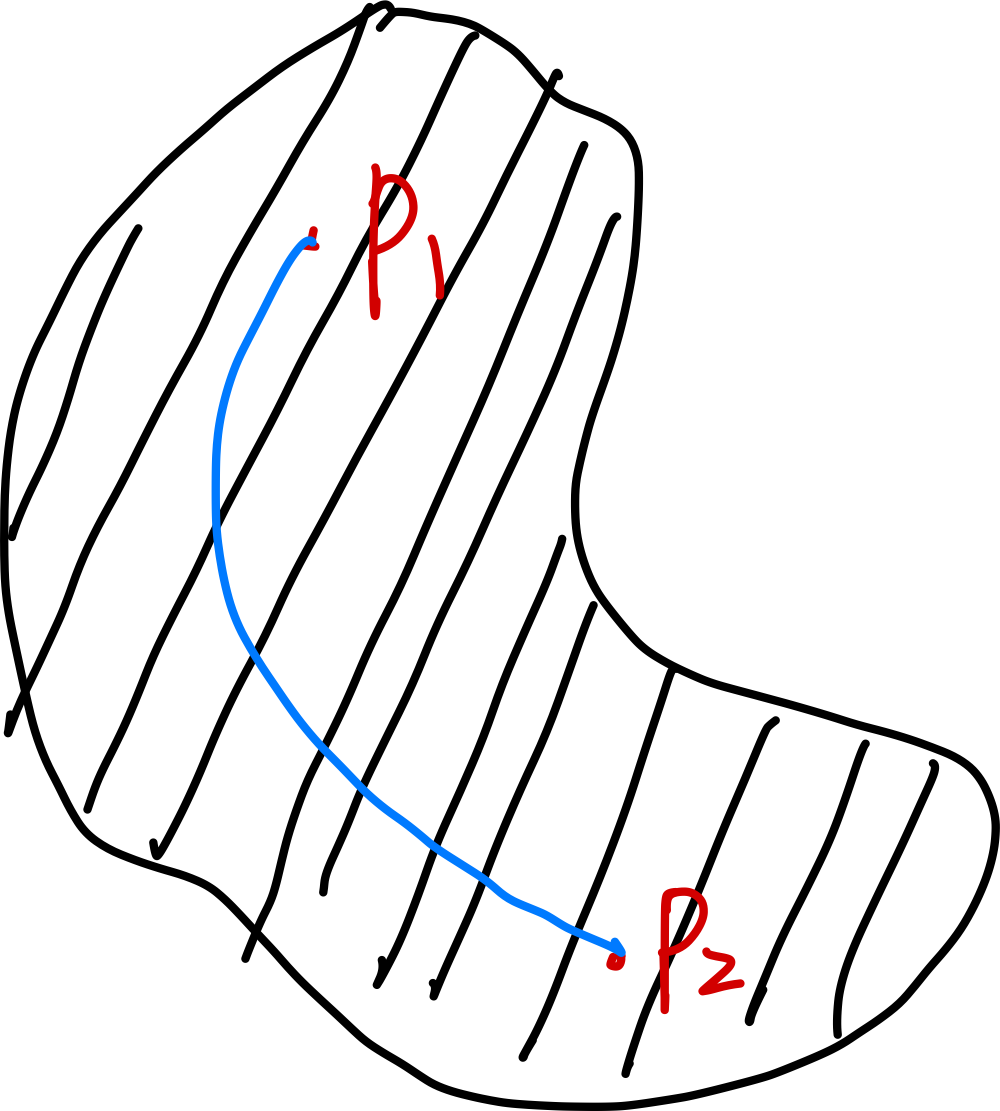
\includegraphics[scale=0.15]{"Chapter 04 images/pic1.png"}
        % \caption{}
        \label{pic4-1}
    \end{wrapfigure}

    角坐标\(\theta = \theta\left(t\right)\),沿逆时针方向转动为\(\theta > 0\),
    角位移\(\Delta \theta = \theta \left(t + \Delta t\right) - \theta\left(t\right)\)。
    角速度矢量

    \begin{equation}
        \omega=\lim _{\Delta t \rightarrow 0} \frac{\Delta \theta}{\Delta t}=\frac{\mathrm{d} \theta}{\mathrm{~d} t}
    \end{equation}

    方向按右手螺旋法则确定。

\subsubsection{刚体定轴转动}

    刚体定轴转动(一维转动)的转动方向可以用角速度的正、负来表示。

    角加速度

    $$
        \overrightarrow{\alpha} = \deriv{\overrightarrow{\omega}}{t}
    $$

    定轴转动的特点:

    \begin{enumerate}
        \item 每一质点均做圆周运动,与轴垂直的圆面为转动平面;
        \item 任意质点运动\(\Delta \theta,\; \omega,\; \overrightarrow{\omega},\; \overrightarrow{\alpha}\)相同,但\(\overrightarrow{v},\; \overrightarrow{a}\)不相同;
        \item 运动描述仅需一个坐标。
    \end{enumerate}

    匀变速转动公式:

    $$
    \begin{array}{|l|l|}
    \hline \text { 质点匀变速直线运动 } & \text { 刚体绕定轴匀变速转动 } \\
    \hline v=v_0+a t & \omega=\omega_0+\alpha t \\
    \hline x=x_0+v_0 t+\frac{1}{2} a t^2 & \theta=\theta_0+\omega_0 t+\frac{1}{2} \alpha t^2 \\
    \hline v^2=v_0^2+2 a\left(x-x_0\right) & \omega^2=\omega_0^2+2 \alpha\left(\theta-\theta_0\right) \\
    \hline
    \end{array}
    $$

    角量与线量的关系:

    \begin{wrapfigure}{r}{4cm}
        \centering
        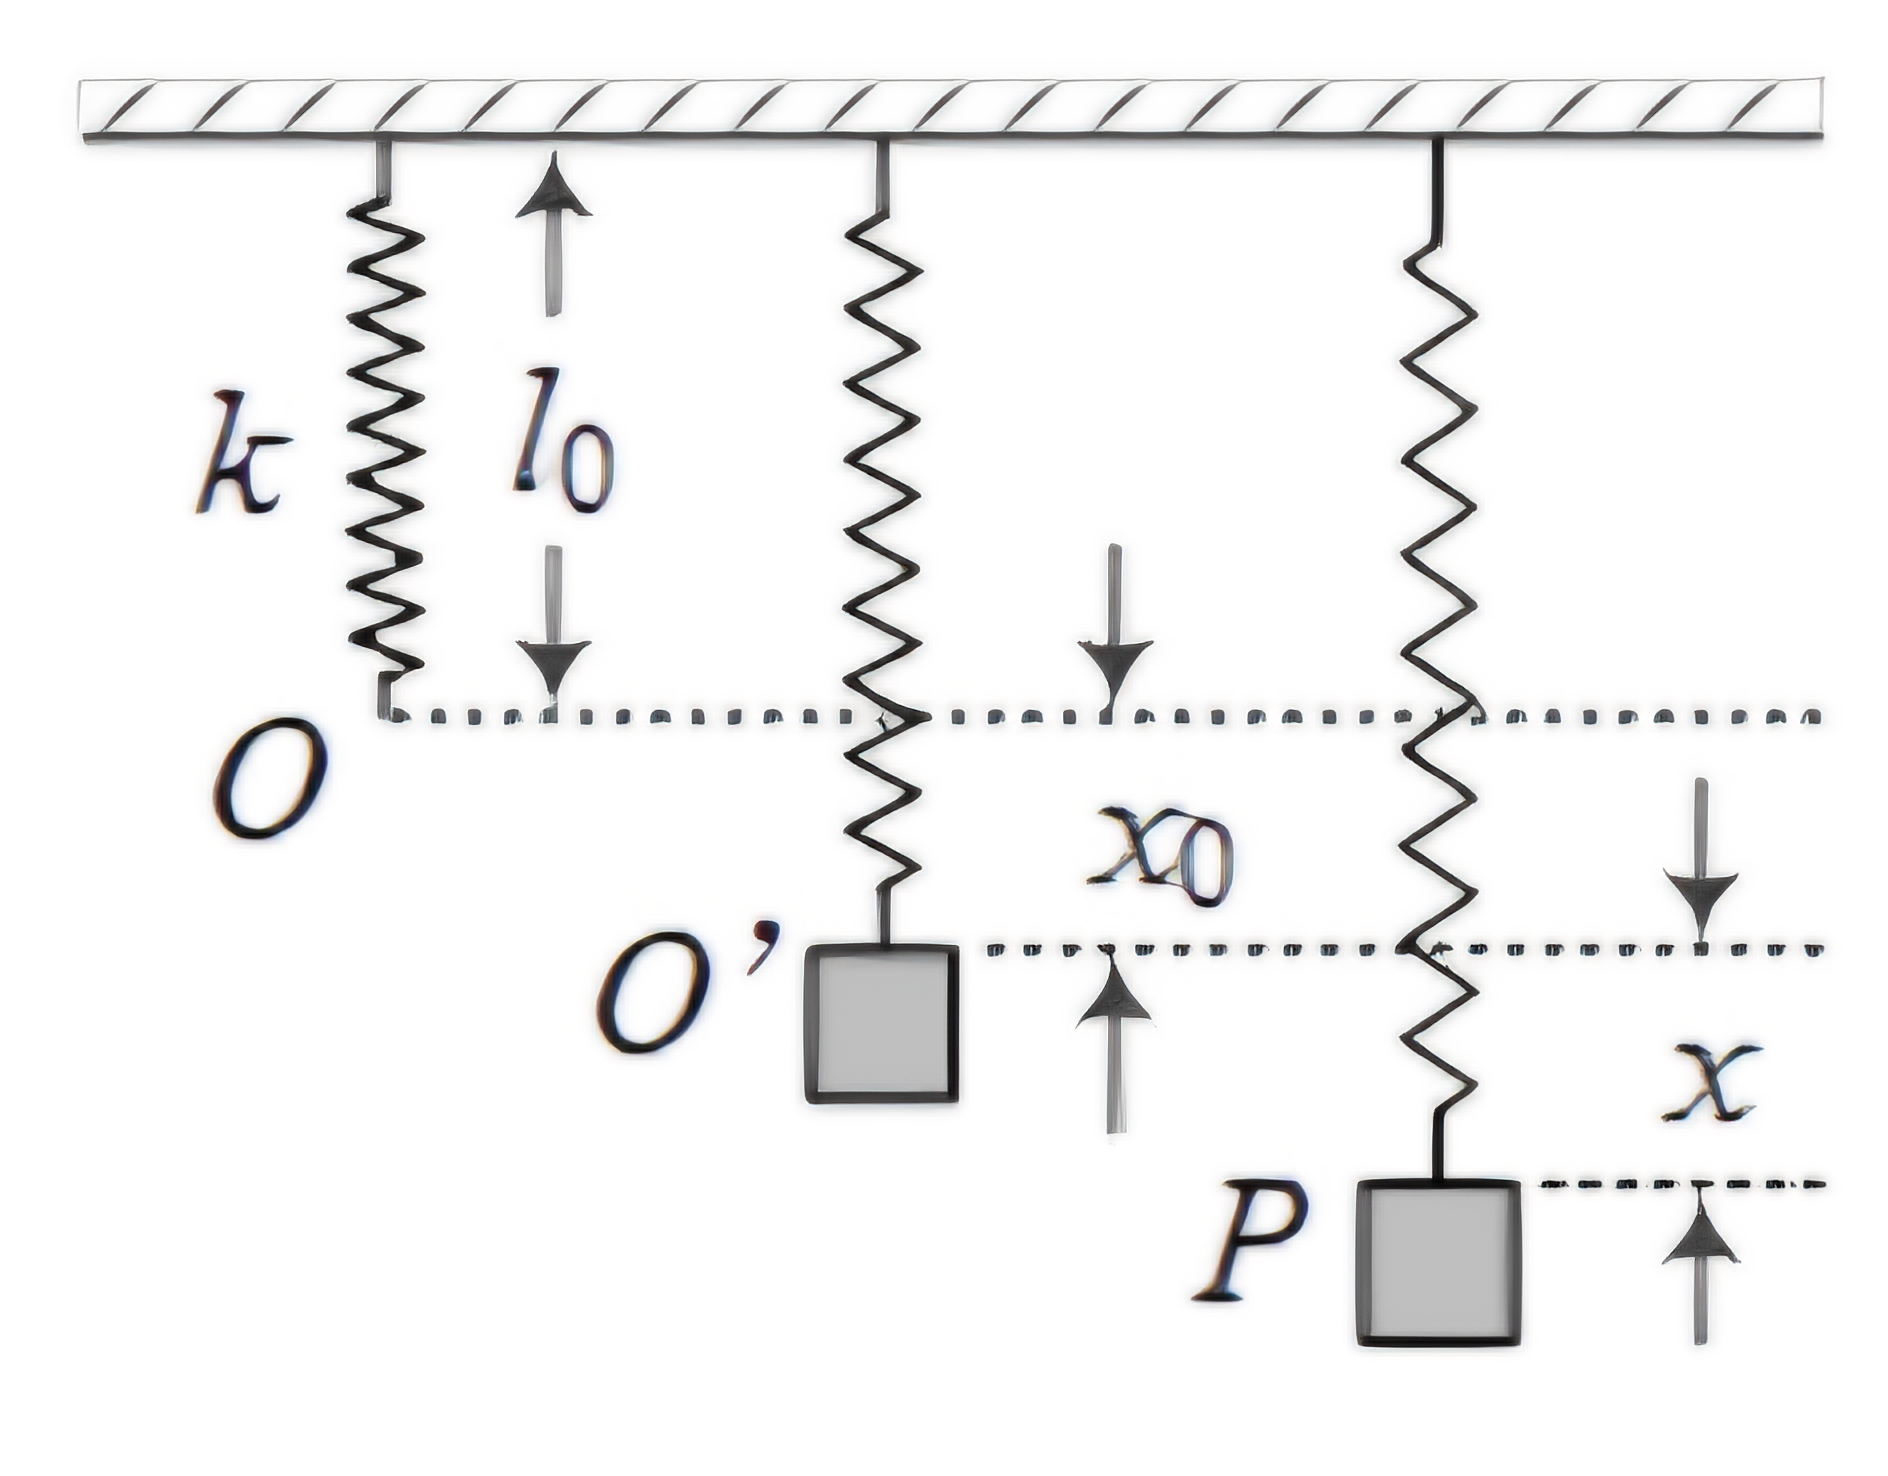
\includegraphics[scale=0.2]{"Chapter 04 images/pic2.png"}
        % \caption{}
        \label{pic4-2}
    \end{wrapfigure}

    \[
        \omega = \deriv{\theta}{t}
    \]

    \[
        \overrightarrow{v_i} = r_i \omega \overrightarrow{e}_t
    \]

    $$
        \overrightarrow{v}=\overrightarrow{\omega} \times \overrightarrow{r}_{\perp}=
        \overrightarrow{\omega} \times \overrightarrow{r}
    $$

    $$
        \alpha=\deriv{\omega}{t}=\frac{\rmd^2 \theta}{\rmd^2 t}
    $$

    于是

    \begin{equation}
        \overrightarrow{a}=r \alpha \overrightarrow{e}_{\mathrm{t}}+r \omega^2 \overrightarrow{e}_{\mathrm{n}}
    \end{equation}

\subsection{力矩}

\subsubsection{定义}

    用来描述力对刚体的转动的作用的物理量。

    \begin{wrapfigure}{r}{4cm}
        \centering
        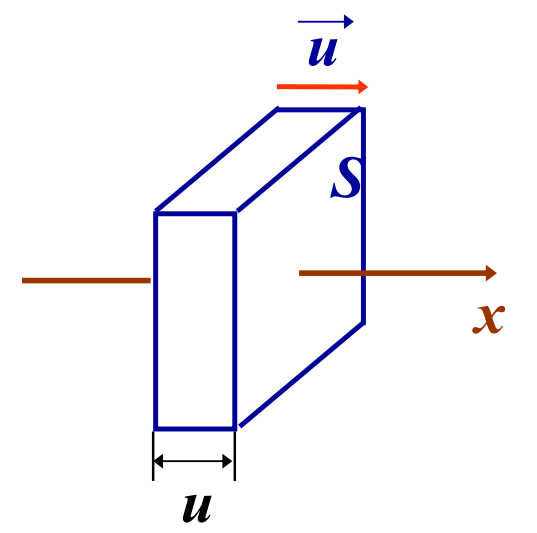
\includegraphics[scale=0.2]{"Chapter 04 images/pic3.png"}
        % \caption{}
        \label{pic4-3}
    \end{wrapfigure}

    刚体绕\(Oz\)轴旋转 , 力作用在刚体上点\(P\),且在转动平面内,为由点\(O\)到力的作用点\(P\)的径矢。
    \(\overrightarrow{F}\)对转轴\(z\)的力矩的定义:

    \begin{align}
        \overrightarrow{M} = \overrightarrow{r} \times \overrightarrow{F}
    \end{align}

    $$
        M = Fr\sin\theta = Fd \quad (d\text{为力臂})
    $$

\subsubsection{讨论}

    \begin{enumerate}
        \item 若力\(\overrightarrow{F}\)不在转动平面内,可将力分解为平行和垂直于转轴方向的两个分量;
        \item 合力矩等于各分力矩的矢量和;
        \item 刚体内作用力和反作用力的力矩相互抵消;
        \item 力矩的单位只能用\(\text{牛顿} \cdot \text{米}\),而不能用焦耳。
    \end{enumerate}

\section{转动定律、转动惯量}

\subsection{质点的转动惯量}

    单个质点\(m\)与转轴刚性连接

    \begin{wrapfigure}{r}{4cm}
        \centering
        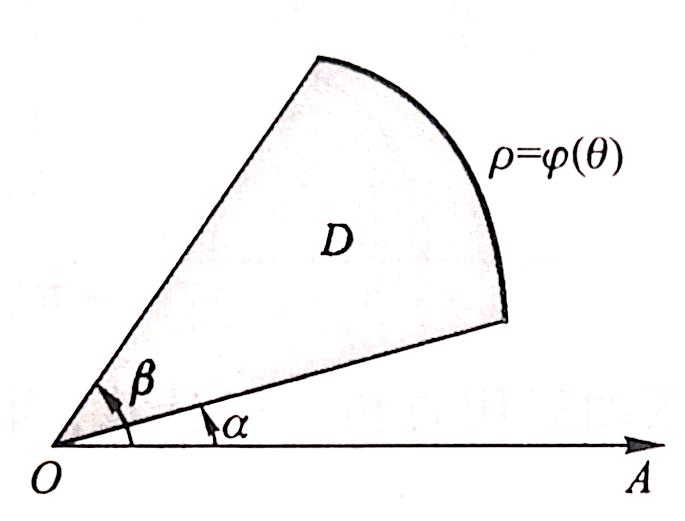
\includegraphics[scale=0.2]{"Chapter 04 images/pic4.png"}
        % \caption{}
        \label{pic4-4}
    \end{wrapfigure}

    $$
        F_{\mathrm{t}}=m a_{\mathrm{t}}=m r \alpha
    $$

    则

    \begin{equation}
        F_{\mathrm{t}}=m a_{\mathrm{t}}=m r \alpha
    \end{equation}

    \textbf{定义}

    \begin{align}
        I = mr^2
    \end{align}

    为质点\(m\)对\(O\)点的“转动惯量”。

    于是

    \begin{align}
        M = I \alpha
    \end{align}

\subsection{刚体的转动惯量}

\subsubsection{定义}

    \begin{wrapfigure}{r}{4cm}
        \centering
        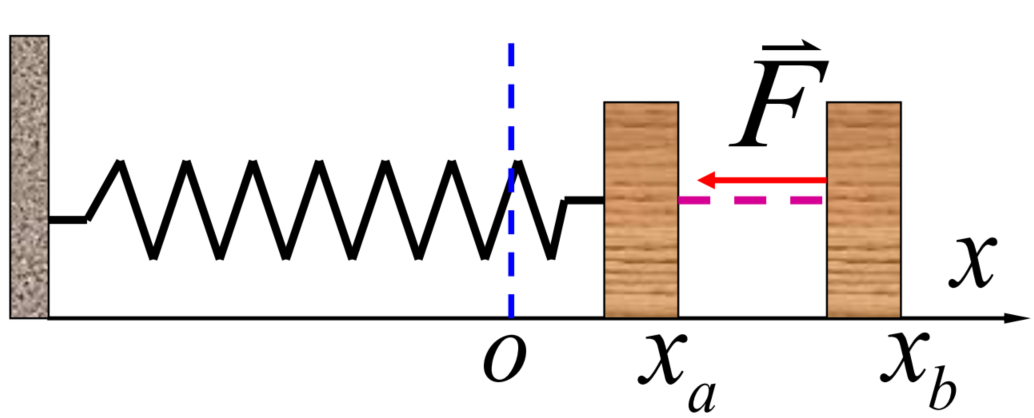
\includegraphics[scale=0.2]{"Chapter 04 images/pic5.png"}
        % \caption{}
        \label{pic4-5}
    \end{wrapfigure}

    质量元受外力\(\overrightarrow{F}_{\mathrm{e}j}\),内力\(\overrightarrow{F}_{\mathrm{i}j}\)

    则

    \begin{align*}
        M_{\mathrm{e} j}+M_{\mathrm{i} j}=\Delta m_j r_j^2 \alpha
    \end{align*}

    因为$M_{i j}=-M_{j i}$,所以

    $$
        \sum_j M_{i j}=0
    $$

    于是

    \begin{equation}
        \sum_j M_{\mathrm{e} j}=\left(\sum \Delta m_j r_j^2\right) \alpha
    \end{equation}

    于是\textbf{定义}

    \begin{align}
        I=\sum_j \Delta m_j r_j^2
    \end{align}

    为刚体对\(O\)点的“转动惯量”。

    积分形式即为

    \begin{equation}
        I=\int r^2 \mathrm{~d} m
    \end{equation}

\subsubsection{几种常见刚体的转动惯量}

    \begin{wrapfigure}{r}{4cm}
        \centering
        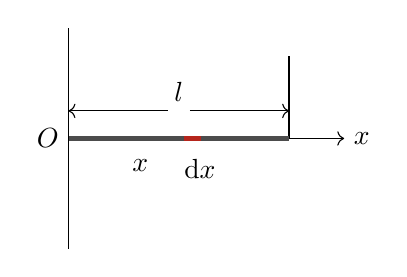
\begin{tikzpicture}[scale=0.7]
            \coordinate[label=left:$O$] (O) at (0,0);
            \coordinate[label=right:$x$] (x_axis) at (5,0);
            \coordinate[label=below:$x$] (x) at (1.3,-0.2);
            \coordinate[label=$l$] (l) at (2,0.5);
            \coordinate[label=below:$\rmd x$] (x) at (2.3,-0.2);
            \draw (0,-2) -- (0,2);
            \draw[->] (O) -- (x_axis);
            \draw (4,0) -- (4,1.5);
            \draw[->] (1.8,0.5) -- (0,0.5);
            \draw[->] (2.2,0.5) -- (4,0.5);
            \draw[line width=2pt, color=black!70] (O) -- (4,0);
            \draw[line width=2pt, color=BrickRed] (2.1,0) -- (2.4,0);
        \end{tikzpicture}
    \end{wrapfigure}

    \textbf{例1 \quad}均匀杆\(m\)对\(O\)轴(通过杆的端点与杆垂直)的转动惯量:

    运用微积分的思想和方法,

    \begin{align*}
        I_{O} = \int x^2 \rmd m = \int_{0}^{l} x^2 \rmd x \lambda = \frac{\lambda l^3}{3} = \frac{1}{3} m l^2
    \end{align*}
    \vspace{1em}

    \begin{wrapfigure}{r}{4cm}
        \centering
        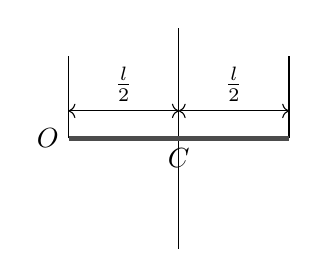
\begin{tikzpicture}[scale=0.7]
            \coordinate[label=left:$O$] (O) at (0,0);
            \coordinate[label=below:$C$] (C) at (2,0);
            \coordinate[label=above:$\frac{l}{2}$] (l-1) at (1,0.5);
            \coordinate[label=above:$\frac{l}{2}$] (l-2) at (3,0.5);
            \draw (O) -- (0,1.5);
            \draw (4,0) -- (4,1.5);
            \draw (2,-2) -- (2,2);
            \draw[<->] (2,0.5) -- (0,0.5);
            \draw[<->] (2,0.5) -- (4,0.5);
            \draw[line width=2pt, color=black!70] (O) -- (4,0);
        \end{tikzpicture}
    \end{wrapfigure}

    \textbf{例2 \quad}均匀杆\(m\)对\(C\)轴(通过杆的端点与杆垂直)的转动惯量:

    $$
        I_C =\frac{1}{12} m l^2
    $$

    \textbf{证}(方法1)

    $$
        \begin{aligned}
            I_C &=\int x^2 \rmd m \\
            &=\int_{-\frac{l}{2}}^{\frac{l}{2}} x^2 d x \lambda\\
            &=\frac{1}{12} \lambda l^3\\
            &=\frac{1}{12} m l^2
        \end{aligned}
    $$

    \textbf{证}(方法2:平行轴定理)

    由平行轴定理,

    $$
        I_O = I_C + m \left(\frac{l}{2}\right)^2
    $$

    于是

    $$
        \begin{aligned}
            I_C &=I_O - m \left(\frac{l}{2}\right)^2 \\
            &=\frac{1}{3} m l^2 - m \left(\frac{l}{2}\right)^2 \\
            &=\frac{1}{12} m l^2
        \end{aligned}
    $$

    \vspace{2em}

    \begin{wrapfigure}{r}{4cm}
        \centering
        \tikzset{every picture/.style={line width=0.75pt}} %set default line width to 0.75pt        
        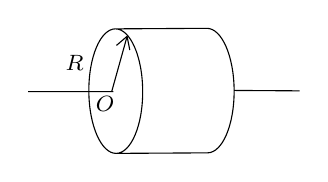
\begin{tikzpicture}[x=0.75pt,y=0.75pt,yscale=-1,xscale=1]
            %uncomment if require: \path (0,300); %set diagram left start at 0, and has height of 300
            %Shape: Can [id:dp17410052803948828] 
            \draw   (167.4,90.33) -- (211.46,90.07) .. controls (218.62,90.03) and (224.5,103.43) .. (224.6,120) ..
                controls (224.69,136.57) and (218.96,150.03) .. (211.8,150.07) -- (167.74,150.33) .. controls
                (160.58,150.37) and (154.7,136.97) .. (154.6,120.4) .. controls (154.51,103.83) and (160.24,90.37) .. (167.4,90.33) ..
                controls (174.56,90.29) and (180.45,103.68) .. (180.54,120.25) .. controls (180.64,136.82) and (174.91,150.29) .. (167.74,150.33) ;
            %Straight Lines [id:da06354151922433426] 
            \draw    (125.4,120.6) -- (166.38,120.54) ;
            %Straight Lines [id:da03453199583434419] 
            \draw    (224.6,120) -- (256.2,120.2) ;
            \draw   (167.91,98.31) -- (173.02,93.94) -- (174.33,100.53) ;
            %Straight Lines [id:da7464924546039589] 
            \draw    (165.62,120.54) -- (173,94.08) ;
            % Text Node
            \draw (156.77,121.4) node [anchor=north west][inner sep=0.75pt]  [font=\footnotesize]  {$O$};
            % Text Node
            \draw (142.15,101.63) node [anchor=north west][inner sep=0.75pt]  [font=\footnotesize]  {$R$};
        \end{tikzpicture}
    \end{wrapfigure}

    \textbf{例3 \quad}均匀圆柱\(m\)对转轴(圆柱体的轴线)的转动惯量:

    $$
        I = \frac{1}{2} m R^2
    $$
    \vspace{2em}

    \begin{wrapfigure}{r}{4cm}
        \centering
        \tikzset{every picture/.style={line width=0.75pt}} %set default line width to 0.75pt        
        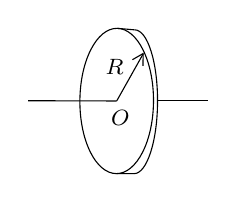
\begin{tikzpicture}[x=0.75pt,y=0.75pt,yscale=-1,xscale=1]
        %uncomment if require: \path (0,300); %set diagram left start at 0, and has height of 300
        %Shape: Ellipse [id:dp023285849196069686] 
        \draw   (169.6,97.35) .. controls (159.81,97.3) and (151.94,81.59) .. (152.04,62.26)
            .. controls (152.13,42.93) and (160.15,27.3) .. (169.94,27.35) .. controls (179.73,27.39) and (187.59,43.1)
            .. (187.5,62.43) .. controls (187.41,81.76) and (179.39,97.39) .. (169.6,97.35) -- cycle ;
        %Shape: Arc [id:dp152216816696912] 
        \draw  [draw opacity=0] (178.39,28.08) .. controls (178.41,28.08) and (178.43,28.08) ..
            (178.45,28.08) .. controls (184.62,28.11) and (189.55,43.64) .. (189.45,62.78) .. controls
            (189.36,81.88) and (184.3,97.35) .. (178.14,97.37) -- (178.28,62.72) -- cycle ;
        \draw (178.39,28.08) .. controls (178.41,28.08) and (178.43,28.08) .. (178.45,28.08) ..
            controls (184.62,28.11) and (189.55,43.64) .. (189.45,62.78) .. controls (189.36,81.88) and (184.3,97.35) .. (178.14,97.37) ;  
        %Straight Lines [id:da15998039992585622] 
        \draw    (169.94,27.35) -- (178.39,28.08) ;
        %Straight Lines [id:da9421417261902603] 
        \draw    (169.6,97.35) -- (178.14,97.37) ;
        %Straight Lines [id:da023543911373016257] 
        \draw    (127.15,62.23) -- (169.77,62.35) ;
        %Straight Lines [id:da05591836369536707] 
        \draw    (189.77,62.23) -- (213.77,62.23) ;
        %Straight Lines [id:da23564039281617188] 
        \draw    (169.77,62.35) -- (182.54,39.62) ;
        \draw   (177.34,42.47) -- (182.49,39.5) -- (182.45,45.45) ;
        % Text Node
        \draw (163.23,41.28) node [anchor=north west][inner sep=0.75pt]  [font=\footnotesize]  {$R$};
        % Text Node
        \draw (165.85,65.74) node [anchor=north west][inner sep=0.75pt]  [font=\footnotesize]  {$O$};
        \end{tikzpicture}
    \end{wrapfigure}

    \textbf{例4 \quad}均匀圆盘\(m\)对转轴(通过盘心垂直于盘面)的转动惯量:

    $$
        I = \frac{1}{2} m R^2
    $$

    \textbf{证}(方法1)

    \[
        \tikzset{every picture/.style={line width=0.75pt}} %set default line width to 0.75pt        
        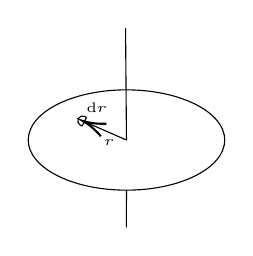
\begin{tikzpicture}[x=0.75pt,y=0.75pt,yscale=-1,xscale=1]
        %uncomment if require: \path (0,300); %set diagram left start at 0, and has height of 300
        %Shape: Ellipse [id:dp6022616866424968] 
        \draw   (213,137.17) .. controls (213,123.82) and (234.19,113) .. (260.33,113) .. controls (286.47,113) and (307.67,123.82) .. (307.67,137.17) .. 
            controls (307.67,150.51) and (286.47,161.33) .. (260.33,161.33) .. controls (234.19,161.33) and (213,150.51) .. (213,137.17) -- cycle ;
        %Straight Lines [id:da33799420686761406] 
        \draw    (260.33,137.17) -- (259.89,83.31) ;
        %Straight Lines [id:da8541013949511429] 
        \draw    (260.29,179.31) -- (260.33,161.33) ;
        %Straight Lines [id:da3324794336188084] 
        \draw    (260.33,137.17) -- (241.12,128.77) ;
        \draw [shift={(239.29,127.96)}, rotate = 23.62] [color={rgb, 255:red, 0; green, 0; blue, 0 }  ][line width=0.75]
            (10.93,-3.29) .. controls (6.95,-1.4) and (3.31,-0.3) .. (0,0) .. controls (3.31,0.3) and (6.95,1.4) .. (10.93,3.29)   ;
        %Shape: Chord [id:dp96440595365312] 
        \draw   (238.98,130.36) .. controls (238.71,130.32) and (238.44,130.24) .. (238.18,130.11) .. controls (236.97,129.48) and (236.48,128.01)
            .. (237.09,126.83) .. controls (237.7,125.65) and (239.18,125.2) .. (240.39,125.82) .. controls (240.65,125.96) and (240.87,126.13) .. (241.06,126.33) -- cycle ;
        % Text Node
        \draw (239.86,117.95) node [anchor=north west][inner sep=0.75pt]  [font=\tiny]  {$\mathrm{d} r$};
        \draw (248.36,135.7) node [anchor=north west][inner sep=0.75pt]  [font=\tiny]  {$r$};
        \end{tikzpicture}
    \]

    设圆盘的面密度为\(\sigma\),则\(\sigma = \dfrac{m}{\uppi R^2}\)

    如图,取微元\(\rmd m\):

    \[
        \tikzset{every picture/.style={line width=0.75pt}} %set default line width to 0.75pt        
        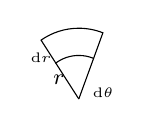
\begin{tikzpicture}[x=0.75pt,y=0.75pt,yscale=-1,xscale=1]
        %uncomment if require: \path (0,300); %set diagram left start at 0, and has height of 300
        %Shape: Block Arc [id:dp4642247634663095] 
        \draw   (206.87,95.84) .. controls (212.07,92.22) and (218.33,90.11) .. (225.06,90.11) .. controls (229.14,90.11) and (233.06,90.89)
            .. (236.66,92.31) -- (232.18,104.64) .. controls (229.97,103.72) and (227.57,103.22) .. (225.06,103.22) .. controls (220.94,103.22)
            and (217.11,104.57) .. (213.95,106.88) -- cycle ;
        %Straight Lines [id:da4857653535391253] 
        \draw    (232.18,104.64) -- (225.06,124.2) ;
        %Straight Lines [id:da18026998140759942] 
        \draw    (213.95,106.88) -- (225.06,124.2) ;
        % Text Node
        \draw (211.49,111.51) node [anchor=north west][inner sep=0.75pt]  [font=\footnotesize]  {$r$};
        \draw (200.69,100.71) node [anchor=north west][inner sep=0.75pt]  [font=\tiny]  {$\mathrm{d} r$};
        \draw (230.62,117.82) node [anchor=north west][inner sep=0.75pt]  [font=\tiny]  {$\mathrm{d} \theta $};
        \end{tikzpicture}
    \]

    则

    \[
        \rmd m = \sigma r \rmd \theta \rmd r
    \]

    于是

    $$
        \begin{aligned}
            I & =\int r^2 \rmd m\\
            & =\int r^2 \sigma r \rmd \theta \rmd r \\
            & =\iint \sigma r^3 \rmd r \rmd \theta \\
            & =\sigma \int_0^R r^3 \rmd r \int_0^{2 \uppi} \rmd \theta \\
            & =\sigma \frac{1}{4} R^4 \cdot 2 \uppi \\
            & =\frac{1}{2} m R^2
        \end{aligned}
    $$

    \textbf{证}(方法2)

    \[
        \tikzset{every picture/.style={line width=0.75pt}} %set default line width to 0.75pt        
        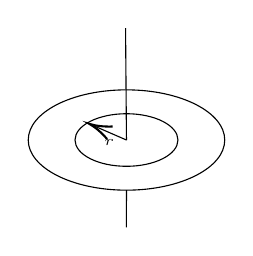
\begin{tikzpicture}[x=0.75pt,y=0.75pt,yscale=-1,xscale=1]
        %uncomment if require: \path (0,300); %set diagram left start at 0, and has height of 300
        %Shape: Ellipse [id:dp6022616866424968] 
        \draw   (213,137.17) .. controls (213,123.82) and (234.19,113) .. (260.33,113) .. controls (286.47,113) and (307.67,123.82)
            .. (307.67,137.17) .. controls (307.67,150.51) and (286.47,161.33) .. (260.33,161.33) .. controls (234.19,161.33) and (213,150.51) .. (213,137.17) -- cycle ;
        %Straight Lines [id:da33799420686761406] 
        \draw    (260.33,137.17) -- (259.89,83.31) ;
        %Straight Lines [id:da8541013949511429] 
        \draw    (260.29,179.31) -- (260.33,161.33) ;
        %Straight Lines [id:da3324794336188084] 
        \draw    (260.33,137.17) -- (244.12,130.12) ;
        \draw [shift={(242.29,129.32)}, rotate = 23.49] [color={rgb, 255:red, 0; green, 0; blue, 0 }  ][line width=0.75] (10.93,-3.29) .. controls
            (6.95,-1.4) and (3.31,-0.3) .. (0,0) .. controls (3.31,0.3) and (6.95,1.4) .. (10.93,3.29)   ;
        %Shape: Ellipse [id:dp4379584317489489] 
        \draw   (235.53,137.17) .. controls (235.53,130.17) and (246.64,124.5) .. (260.33,124.5) .. controls (274.03,124.5) and
            (285.13,130.17) .. (285.13,137.17) .. controls (285.13,144.16) and (274.03,149.83) .. (260.33,149.83) .. controls (246.64,149.83) and (235.53,144.16) .. (235.53,137.17) -- cycle ;
        % Text Node
        \draw (248.36,135.7) node [anchor=north west][inner sep=0.75pt]  [font=\tiny]  {$r$};
        \end{tikzpicture}
    \]

    同样,设圆盘的面密度为\(\sigma = \dfrac{m}{\uppi R^2}\)。取距离圆心\(r\)的某一圆环
    (宽\(\rmd r\))为\(\rmd m\),则

    \[
        \rmd m = \sigma 2 \uppi r \rmd r
    \]

    于是

    $$
        \begin{aligned}
            I &= \int r^2 \rmd m \\
            &= \int_{0}^{R} r^2 \cdot \sigma 2 \uppi r \rmd r \\
            & =\frac{1}{2} m R^2
        \end{aligned}
    $$

    \begin{wrapfigure}{r}{4cm}
        \centering
        \tikzset{every picture/.style={line width=0.75pt}} %set default line width to 0.75pt        
        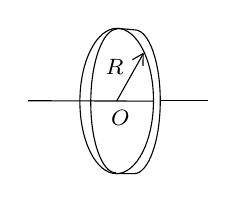
\begin{tikzpicture}[x=0.75pt,y=0.75pt,yscale=-1,xscale=1]
        %uncomment if require: \path (0,300); %set diagram left start at 0, and has height of 300
        %Shape: Ellipse [id:dp023285849196069686] 
        \draw   (169.6,97.35) .. controls (159.81,97.3) and (151.94,81.59) .. (152.04,62.26) ..
            controls (152.13,42.93) and (160.15,27.3) .. (169.94,27.35) .. controls (179.73,27.39) and (187.59,43.1)
            .. (187.5,62.43) .. controls (187.41,81.76) and (179.39,97.39) .. (169.6,97.35) -- cycle ;
        %Shape: Arc [id:dp152216816696912] 
        \draw  [draw opacity=0] (178.39,28.08) .. controls (178.41,28.08) and (178.43,28.08) .. (178.45,28.08)
            .. controls (185.34,28.11) and (190.86,43.65) .. (190.76,62.78) .. controls (190.67,81.89) and (185.02,97.36)
            .. (178.14,97.37) -- (178.28,62.72) -- cycle ; \draw   (178.39,28.08) .. controls (178.41,28.08) and (178.43,28.08)
            .. (178.45,28.08) .. controls (185.34,28.11) and (190.86,43.65) .. (190.76,62.78) .. controls (190.67,81.89) and (185.02,97.36) .. (178.14,97.37) ;  
        %Straight Lines [id:da15998039992585622] 
        \draw    (169.94,27.35) -- (178.39,28.08) ;
        %Straight Lines [id:da9421417261902603] 
        \draw    (169.6,97.35) -- (178.14,97.37) ;
        %Straight Lines [id:da023543911373016257] 
        \draw    (127.15,62.23) -- (187.5,62.43) ;
        %Straight Lines [id:da05591836369536707] 
        \draw    (191.31,62.23) -- (213.77,62.23) ;
        %Straight Lines [id:da23564039281617188] 
        \draw    (169.77,62.35) -- (182.54,39.62) ;
        \draw   (177.34,42.47) -- (182.49,39.5) -- (182.45,45.45) ;
        %Shape: Arc [id:dp47532243106850425] 
        \draw  [draw opacity=0] (169.5,96.99) .. controls (169.48,96.99) and (169.46,96.99) ..
            (169.44,96.99) .. controls (162.54,96.93) and (157.1,81.36) .. (157.28,62.23) .. controls (157.47,43.12)
            and (163.19,27.68) .. (170.07,27.7) -- (169.77,62.35) -- cycle ; \draw   (169.5,96.99) ..
            controls (169.48,96.99) and (169.46,96.99) .. (169.44,96.99) .. controls (162.54,96.93) and (157.1,81.36)
            .. (157.28,62.23) .. controls (157.47,43.12) and (163.19,27.68) .. (170.07,27.7) ;  
        % Text Node
        \draw (163.23,41.28) node [anchor=north west][inner sep=0.75pt]  [font=\footnotesize]  {$R$};
        % Text Node
        \draw (165.85,65.74) node [anchor=north west][inner sep=0.75pt]  [font=\footnotesize]  {$O$};
        \end{tikzpicture}
    \end{wrapfigure}

    \textbf{例5 \quad}均匀圆环\(m\)对转轴(通过环心垂直于盘面)的转动惯量:

    $$
        I = m R^2
    $$
    \vspace{2em}

    \begin{wrapfigure}{r}{4cm}
        \centering
        \tikzset{every picture/.style={line width=0.75pt}} %set default line width to 0.75pt        
        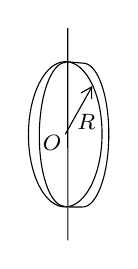
\begin{tikzpicture}[x=0.75pt,y=0.75pt,yscale=-1,xscale=1]
        %uncomment if require: \path (0,300); %set diagram left start at 0, and has height of 300
        %Shape: Ellipse [id:dp023285849196069686] 
        \draw   (169.6,97.35) .. controls (159.81,97.3) and (151.94,81.59) .. (152.04,62.26)
            .. controls (152.13,42.93) and (160.15,27.3) .. (169.94,27.35) .. controls (179.73,27.39) and (187.59,43.1)
            .. (187.5,62.43) .. controls (187.41,81.76) and (179.39,97.39) .. (169.6,97.35) -- cycle ;
        %Shape: Arc [id:dp152216816696912] 
        \draw  [draw opacity=0] (178.39,28.08) .. controls (178.41,28.08) and (178.43,28.08) .. (178.45,28.08) ..
            controls (185.34,28.11) and (190.86,43.65) .. (190.76,62.78) .. controls (190.67,81.89) and (185.02,97.36)
            .. (178.14,97.37) -- (178.28,62.72) -- cycle ; \draw   (178.39,28.08) .. controls (178.41,28.08) and (178.43,28.08)
            .. (178.45,28.08) .. controls (185.34,28.11) and (190.86,43.65) .. (190.76,62.78) .. controls (190.67,81.89)
            and (185.02,97.36) .. (178.14,97.37) ;  
        %Straight Lines [id:da15998039992585622] 
        \draw    (169.94,27.35) -- (178.39,28.08) ;
        %Straight Lines [id:da9421417261902603] 
        \draw    (169.6,97.35) -- (178.14,97.37) ;
        %Straight Lines [id:da23564039281617188] 
        \draw    (169.77,62.35) -- (182.54,39.62) ;
        \draw   (177.34,42.47) -- (182.49,39.5) -- (182.45,45.45) ;
        %Shape: Arc [id:dp47532243106850425] 
        \draw  [draw opacity=0] (169.5,96.99) .. controls (169.48,96.99) and (169.46,96.99) ..
            (169.44,96.99) .. controls (162.54,96.93) and (157.1,81.36) .. (157.28,62.23) ..
            controls (157.47,43.12) and (163.19,27.68) .. (170.07,27.7) -- (169.77,62.35) -- cycle ;
        \draw (169.5,96.99) .. controls (169.48,96.99) and (169.46,96.99) .. (169.44,96.99) ..
            controls (162.54,96.93) and (157.1,81.36) .. (157.28,62.23) .. controls (157.47,43.12) and (163.19,27.68) .. (170.07,27.7) ;  
        %Straight Lines [id:da7330715455990151] 
        \draw    (170.96,11.25) -- (171.04,113.44) ;
        % Text Node
        \draw (174.31,51.43) node [anchor=north west][inner sep=0.75pt]  [font=\footnotesize]  {$R$};
        % Text Node
        \draw (157.69,61.74) node [anchor=north west][inner sep=0.75pt]  [font=\footnotesize]  {$O$};
        \end{tikzpicture}
    \end{wrapfigure}

    \textbf{例6 \quad}均匀圆环\(m\)对转轴(沿圆环直径)的转动惯量:

    $$
        I = \frac{1}{2} m R^2
    $$
    \vspace{4em}

    \begin{wrapfigure}{r}{4cm}
        \centering
        \tikzset{every picture/.style={line width=0.75pt}} %set default line width to 0.75pt        
        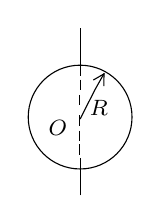
\begin{tikzpicture}[x=0.75pt,y=0.75pt,yscale=-1,xscale=1]
        %uncomment if require: \path (0,300); %set diagram left start at 0, and has height of 300
        %Straight Lines [id:da23564039281617188] 
        \draw    (171,61.56) -- (178.11,47.51) -- (182.54,39.62) ;
        \draw   (177.34,42.77) -- (182.49,39.81) -- (182.45,45.76) ;
        %Straight Lines [id:da7330715455990151] 
        \draw    (171,17.81) -- (171,35.62) ;
        %Shape: Circle [id:dp7000744143017317] 
        \draw   (146,60.62) .. controls (146,46.81) and (157.19,35.62) ..
            (171,35.62) .. controls (184.81,35.62) and (196,46.81) .. (196,60.62) .. controls
            (196,74.42) and (184.81,85.62) .. (171,85.62) .. controls (157.19,85.62)
            and (146,74.42) .. (146,60.62) -- cycle ;
        %Straight Lines [id:da5423143354957887] 
        \draw    (171,98.31) -- (171,85.62) ;
        %Straight Lines [id:da1925163091022266] 
        \draw    (171,35.62) -- (171,40.69) ;
        %Straight Lines [id:da49186666744211105] 
        \draw    (171,42.62) -- (171,47.69) ;
        %Straight Lines [id:da6273845348478542] 
        \draw    (170.88,49.87) -- (170.88,54.94) ;
        %Straight Lines [id:da5600475408875403] 
        \draw    (170.63,59.62) -- (170.63,64.69) ;
        %Straight Lines [id:da3768869837055404] 
        \draw    (170.75,67.12) -- (170.75,72.19) ;
        %Straight Lines [id:da21244422124496465] 
        \draw    (170.88,73.62) -- (170.88,78.69) ;
        %Straight Lines [id:da19418219961056882] 
        \draw    (171,80.54) -- (171,85.62) ;
        % Text Node
        \draw (174.46,51.43) node [anchor=north west][inner sep=0.75pt]  [font=\footnotesize]  {$R$};
        % Text Node
        \draw (154.6,60.92) node [anchor=north west][inner sep=0.75pt]  [font=\footnotesize]  {$O$};
        \end{tikzpicture}
    \end{wrapfigure}

    \textbf{例7 \quad}薄球壳\(m\)对转轴(沿直径)的转动惯量:

    $$
        I = \frac{2}{3} m R^2
    $$
    \vspace{4em}

    \begin{wrapfigure}{r}{4cm}
        \centering
        \tikzset{every picture/.style={line width=0.75pt}} %set default line width to 0.75pt        
        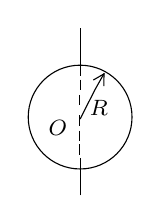
\begin{tikzpicture}[x=0.75pt,y=0.75pt,yscale=-1,xscale=1]
        %uncomment if require: \path (0,300); %set diagram left start at 0, and has height of 300
        %Straight Lines [id:da23564039281617188] 
        \draw (171,61.56) -- (178.11,47.51) -- (182.54,39.62) ;
        \draw (177.34,42.77) -- (182.49,39.81) -- (182.45,45.76) ;
        %Straight Lines [id:da7330715455990151] 
        \draw (171,17.81) -- (171,35.62) ;
        %Shape: Circle [id:dp7000744143017317] 
        \draw (146,60.62) .. controls (146,46.81) and (157.19,35.62) ..
            (171,35.62) .. controls (184.81,35.62) and (196,46.81) .. (196,60.62) .. controls
            (196,74.42) and (184.81,85.62) .. (171,85.62) .. controls (157.19,85.62)
            and (146,74.42) .. (146,60.62) -- cycle ;
        %Straight Lines [id:da5423143354957887] 
        \draw (171,98.31) -- (171,85.62) ;
        %Straight Lines [id:da1925163091022266] 
        \draw (171,35.62) -- (171,40.69) ;
        %Straight Lines [id:da49186666744211105] 
        \draw (171,42.62) -- (171,47.69) ;
        %Straight Lines [id:da6273845348478542] 
        \draw (170.88,49.87) -- (170.88,54.94) ;
        %Straight Lines [id:da5600475408875403] 
        \draw (170.63,59.62) -- (170.63,64.69) ;
        %Straight Lines [id:da3768869837055404] 
        \draw (170.75,67.12) -- (170.75,72.19) ;
        %Straight Lines [id:da21244422124496465] 
        \draw (170.88,73.62) -- (170.88,78.69) ;
        %Straight Lines [id:da19418219961056882] 
        \draw (171,80.54) -- (171,85.62) ;
        % Text Node
        \draw (174.46,51.43) node [anchor=north west][inner sep=0.75pt]  [font=\footnotesize]  {$R$};
        % Text Node
        \draw (154.6,60.92) node [anchor=north west][inner sep=0.75pt]  [font=\footnotesize]  {$O$};
        \end{tikzpicture}
    \end{wrapfigure}

    \textbf{例8 \quad}均匀实心球体\(m\)对转轴(沿直径)的转动惯量:

    $$
        I = \frac{2}{5} m R^2
    $$
    \vspace{2em}

\subsection{转动定律}

\subsubsection{定律}

    \begin{align}
        M = I \alpha
    \end{align}

\subsubsection{讨论}

    \begin{enumerate}
        \item 若\(M=0\),则\(\alpha=0\),即\(\omega\)不变;
        \item \(\alpha \)与\(\frac{M}{I}\)成反比;
        \item \(M = I\alpha = I\deriv{\omega}{t}\);
        \item 转动惯量的单位为\(\mathrm{kg} \cdot \mathrm{m^2}\);
        \item 转动惯量的是对某一转轴而言的;
        \item 转动惯量是转动惯性的量度;
        \item 转动惯量具有可叠加性;
        \item 转动惯量与刚体的质量、质量的分布以及转轴的位置有关。
    \end{enumerate}

\subsubsection{平行轴定理}

    \begin{wrapfigure}{r}{4cm}
        \centering
        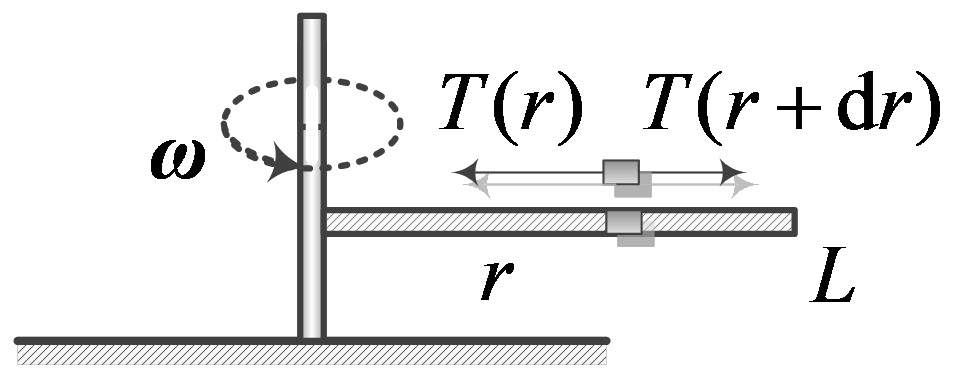
\includegraphics[scale=0.2]{"Chapter 04 images/pic6.png"}
        % \caption{}
        \label{pic4-6}
    \end{wrapfigure}

    质量为\(m\)的刚体,如果对其质心轴的转动惯量为\(I_{C}\),则对任一与该轴平行,
    相对\(d\)的转轴的转动惯量

    \begin{align}
        I = I_{C} + md^2
    \end{align}

\subsubsection{垂直轴定理(正交轴定理)}

    对\textbf{薄板状}刚体:对板面内相互垂直的两个定轴的转动惯量之和
    等于该刚体对通过两轴交点且垂直于板面的定轴的转动惯量。

    \begin{align}
        I_{z} = I_{x} + I_{y}
    \end{align}

    证明:

    \begin{align*}
        \begin{aligned}
            I_{z} &= \sum \Delta m_{i}r_{i}^2 \\
            &= \sum \Delta m_{i}\left(x_{i}^2 + y_{i}^2\right) \\
            &= I_{x} + I_{y}
        \end{aligned}
    \end{align*}

\subsection{例题}

\subsubsection{problem 1}

    \begin{wrapfigure}{r}{4cm}
        \centering
        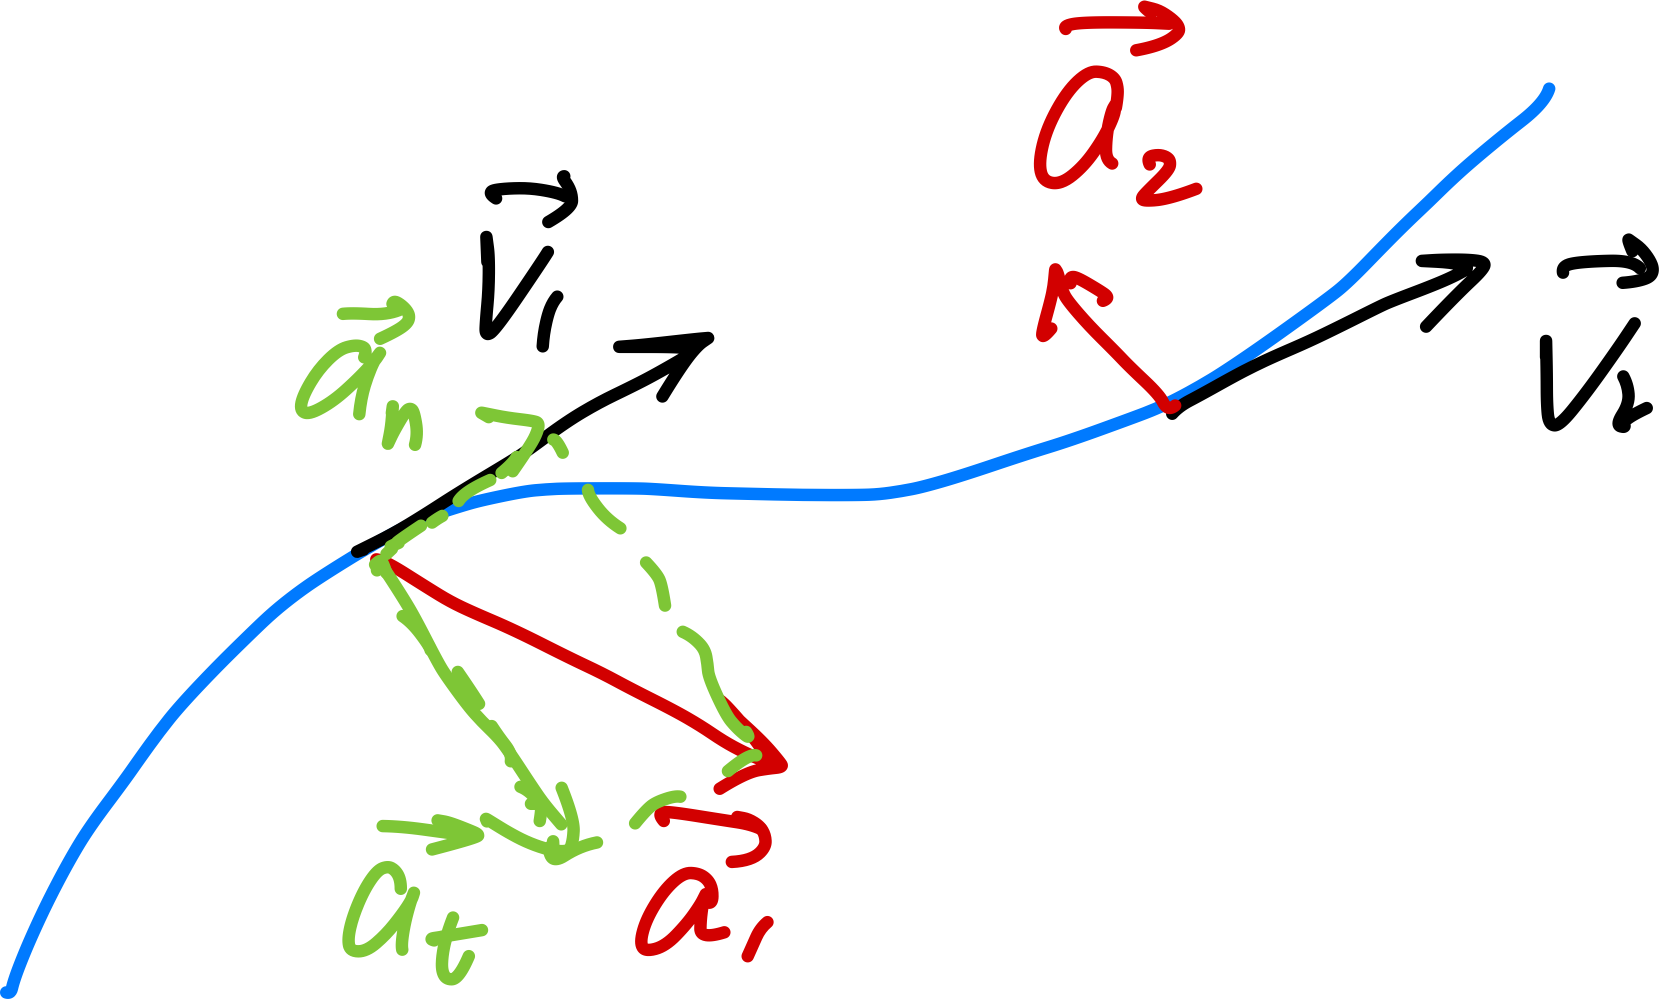
\includegraphics[scale=0.2]{"Chapter 04 images/pic7.png"}
        % \caption{}
        \label{pic4-7}
    \end{wrapfigure}

    质量为\(M\)的匀质圆盘,可绕通过盘中心并垂直于盘面的固定光滑轴转动,转动惯量为
    \(\frac{1}{2}Mr^2\)。一根长为\(l\),质量为\(m\)的匀质柔软绳索挂在圆盘上,如图所示。
    设绳与圆盘间无相对滑动,试求当圆盘两侧绳长之差为\(S\)时,绳的加速度的大小。
    \vspace{1em}

    \textbf{Solution}
    \vspace{1em}

    设某一时刻圆盘两侧的绳长分别为\(x_1\)、\(x_2\)(\(x_1 > x_2\)),如图所示。
    可将绳分为三段,即长度分别为\(x1\)、\(x2\)的两段绳和绕在盘上的一段,
    由于绕在盘上的一段谁盘一起转动,所以可将它和盘作为一个整体来讨论。
    假设在 1、2 两点处绳中的张力分别为\(T_1\)、\(T_2\),则由牛顿定律和转动定律可得

    \[
        x_2 \rho g - T_2 = x_2 \rho a
    \]

    \[
        T_1 - x_1 \rho g = x_1 \rho a
    \]

    \[
        T_2r - T_1r = I \alpha
    \]

    且

    \[
        a = r\alpha
    \]

    式中,

    \[
        \rho = \frac{m}{l}
    \]

    是绳的线密度,

    \[
        I = \frac{1}{2}Mr^2 + \uppi r \rho \cdot r^2
    \]

    是绕在盘上的绳与盘作为整体的转动惯量。

    联立以上方程,并取\(x_2-x_1=S\),可得绳的加速度为

    $$
        a=\frac{2 m g S}{(2 m+M) l}
    $$

\section{刚体定轴转动的功能关系}

\subsection{力矩做功}

    \(\overrightarrow{F}\)在转动平面内,

    \begin{equation*}
        \mathrm{d} A=\overrightarrow{F} \cdot \mathrm{~d} \overrightarrow{r}=F_\tau \mathrm{d} s=F_\tau r \mathrm{~d} \theta
        \label{formula-4-3-1}
    \end{equation*}

    上式也可写成

    \begin{equation}
        \mathrm{d} A = M \rmd \theta
    \end{equation}

    于是力矩\(M\)对刚体所做的总功为

    \begin{equation}
        A=\int \mathrm{d} A=\int_{\theta_0}^\theta M \mathrm{~d} \theta
    \end{equation}

    由式\ref{formula-4-3-1}还可得出力矩做功的瞬时功率为

    \begin{equation}
        P=\frac{\mathrm{d} A}{\mathrm{~d} t}=\frac{M \mathrm{~d} \theta}{\mathrm{~d} t}=M \omega
    \end{equation}

    当\(\overrightarrow{M}\)与\(\overrightarrow{\omega}\)同向,\(W\)、\(P\)为正;
    当\(\overrightarrow{M}\)与\(\overrightarrow{\omega}\)反向,\(W\)、\(P\)为负。

\subsection{转动动能}

    整个刚体的动能就是所有质元的动能之和:

    \begin{equation}
        E_{\mathrm{k}}=\sum_i \frac{1}{2} \Delta m_i r_i^2 \omega^2=\frac{1}{2}\left(\sum_i \Delta m_i r_i^2\right) \omega^2
    \end{equation}

    即

    \begin{equation}
        E_{\mathrm{k}}=\frac{1}{2} I \omega^2
    \end{equation}

\subsection{刚体定轴转动的动能定理}

    由

    \begin{equation*}
        A=\int_{\theta_1}^{\theta_2} M \mathrm{~d} \theta=\int_{\theta_1}^{\theta_2} I \frac{\mathrm{~d} \omega}{\mathrm{~d} t} \mathrm{~d} \theta=\int_{\omega_1}^{\omega_2} I \omega \mathrm{~d} \omega
    \end{equation*}

    有

    \begin{equation}
        A=\int_{\theta_1}^{\theta_2} M \mathrm{~d} \theta=\int_{\omega_1}^{\omega_2} I \omega \mathrm{~d} \omega=\frac{1}{2} I \omega_2^2-\frac{1}{2} I \omega_1^2
    \end{equation}

    即:合外力矩对绕定轴转动的刚体所作的功等于刚体转动动能的增量。
    ——刚体绕定轴转动的动能定理

\section{刚体的角动量、角动量定理、角动量守恒定律}

    \textbf{力}的时间累积效应:冲量、动量、动量定理。

    \textbf{力矩}的时间累积效应:冲量矩、角动量、角动量定理。

\subsection{刚体定轴转动的角动量}

\subsubsection{质点的角动量}

    质量为\(m\)的质点以速度\(\overrightarrow{v}\)在空间运动,某时刻对\(O\)的位矢为
    \(\overrightarrow{r}\),则质点对\(O\)的角动量定义为

    \begin{equation}
        \overrightarrow{L} = \overrightarrow{r} \times \overrightarrow{p}
        = \overrightarrow{r} \times m \overrightarrow{v}
    \end{equation}

    \[
        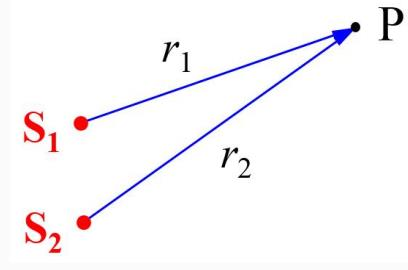
\includegraphics[scale=0.12]{"Chapter 04 images/pic8.png"}
        % \caption{}
        \label{pic4-8}
    \]

    当质点以角速度\(\omega\)作半径为\(r\)的圆运动时,
    相对圆心的角动量:

    \begin{equation}
        L = r m v = r^2 m \omega
    \end{equation}
    
    (方向按右手螺旋法则确定)

\subsubsection{刚体的角动量}

    对于绕\(z\)轴转动的刚体(质点系,每个质点做圆周运动):

    \begin{equation}
        L_z =\sum_i L_{z i}=\sum_i r_i^2 \Delta m_i \omega
        =\left(\sum_i r_i^2 \Delta m_i\right) \omega=I_z \omega
    \end{equation}

\subsection{刚体定轴转动的角动量定理}

\subsubsection{质点的角动量定理}

    \begin{equation}
        \overrightarrow{M} = \deriv{\overrightarrow{L}}{t}
    \end{equation}

    作用于质点的合外力对参考点0的力矩,等于质点对该点\(O\)的角动量随时间的变化率。

    微分形式:

    \begin{equation}
        \overrightarrow{M} \rmd t = \rmd L
    \end{equation}

    积分形式:

    \begin{equation}
        \int_{t_1}^{t_2} \overrightarrow{M} \rmd t = \overrightarrow{L}_2 - \overrightarrow{L}_1
    \end{equation}

    定义\textbf{冲量矩}:

    \begin{equation}
        \int_{t_1}^{t_2} \overrightarrow{M} \rmd t
    \end{equation}

    质点的角动量定理另一表述:对同一参考点\(O\),
    质点所受的冲量矩等于质点角动量的增量。

\subsubsection{质点的角动量守恒定律}

    由质点的角动量定理:

    如果\(\overrightarrow{M}=\overrightarrow{0}\),则

    \begin{equation}
        \overrightarrow{L} = \overrightarrow{r} \times m \overrightarrow{v}
        = \text{恒矢量}
    \end{equation}

    若质点所受外力对某给定点\(O\)的力矩为零,则质点对\(O\)点的角动量保持不变。

\subsubsection{刚体定轴转动的角动量定理}

    刚体也是质点系,刚体定轴转动的角动量定理的微分形式应为

    \begin{equation}
        M \rmd t = \rmd \left(I \omega\right)
    \end{equation}

    \textbf{注意}:这两式对非刚体(转动惯量会发生变化)也成立。

    而刚体绕定轴的转动定律:

    \begin{equation}
        M = I \deriv{\omega}{t}
    \end{equation}

    (\(I\)是常数,仅对刚体成立)

    刚体(非刚体)定轴转动的角动量定理的积分形式:

    \begin{equation}
        \int_{t_1}^{t_2} M \mathrm{~d} t=\int_{\left(I \omega\right)_1}^{\left(I \omega\right)_2} \rmd \left(I \omega\right)
        =I_2 \omega_2-I_1 \omega_1
    \end{equation}

\subsection{刚体定轴转动的角动量守恒定律}

    如果\(\overrightarrow{M}=\overrightarrow{0}\),则

    \begin{equation}
        L = I \omega = \text{常量}
    \end{equation}

    若物体所受的合外力矩为零,则物体的角动量保持不变。

    \begin{enumerate}
        \item 若\(I\)不变,\(\omega\)不变;
        \item 若\(I\)变,\(\omega\)也变,但\(L = I \omega\)不变。
    \end{enumerate}

    即内力矩不改变系统的角动量。

    在冲击等问题中,\(M^{\text{in}} \gg  M^{\text{ex}}\),可认为\(L \approx \text{常量}\)。

\subsection{共轴系统定轴转动的角动量定理}

    当一个系统由多个物体和质点组成时,则某段时间内对某轴
    的合外力矩的冲量矩等于系统绕该轴的角动量的增量:

    $$
    \int_{t_1}^{t_2} M \mathrm{~d} t=\left(\sum_i I_i \omega_i\right)_2-\left(\sum I_i \omega_i\right)_1
    $$

    (\(I_i\)、\(\omega_i\)应对同一轴,\(\omega_i\)应对同一惯性系。)

    共轴系统的定轴转动的角动量守恒定律:

    当系统对某轴的合外力矩的冲量矩等于零时,系统绕该轴的角动量守恒,即:

    \begin{equation}
        \int_{t_1}^{t_2} M \rmd t \text{时,} \sum_{i} I_i \omega_i = \text{恒矢量}
    \end{equation}

    (\(I_i\)、\(\omega_i\)应对同一轴,\(\omega_i\)应对同一惯性系。)

\end{document}
